\startchapter{Dark Matter Searches with the ATLAS Detector}
\label{chapter:theory}

% --------------------------------------------------------------------------------------
\section{Dark Matter Theory}

Effective field theories (EFTs) \cite{Boveia:2016mrp} \cite{Carpenter:2012rg} were the primary models studied in \etmissX dark matter searches in Run 1, when the centre-of-mass energy was 8 TeV. In short, these theories assume that a dark matter pair is produced by means of a contact interaction with a quark and antiquark, as illustrated in Figure \ref{fig:efts}. These types of models offer a straightforward means to compare collider results to direct or indirect detection experiments. However, EFTs are only valid when the mass of the mediating particle between the \chichi and \qq is much heavier than the momentum transfer of the process. Now that the centre-of-mass energy has increased to 13 TeV in Run 2, these EFTs are no longer valid. Thus, a new baseline model is used in Run 2 with the mediator particle explicitly included.

\begin{figure}[htb]
    \centering
    \selectcolormodel{gray}
    \begin{subfigure}[b]{0.35\textwidth}
        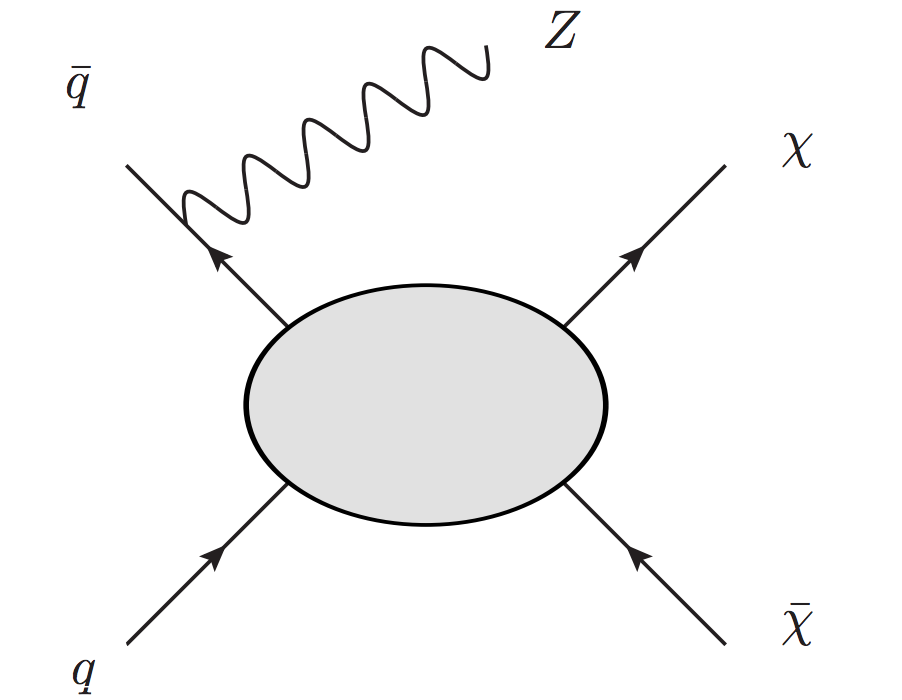
\includegraphics[width=\textwidth]{Figures/eft1.png}
        \label{fig:eft1}
    \end{subfigure}
    ~ %add desired spacing between images, e. g. ~, \quad, \qquad, \hfill etc. 
      %(or a blank line to force the subfigure onto a new line)
    \begin{subfigure}[b]{0.35\textwidth}
        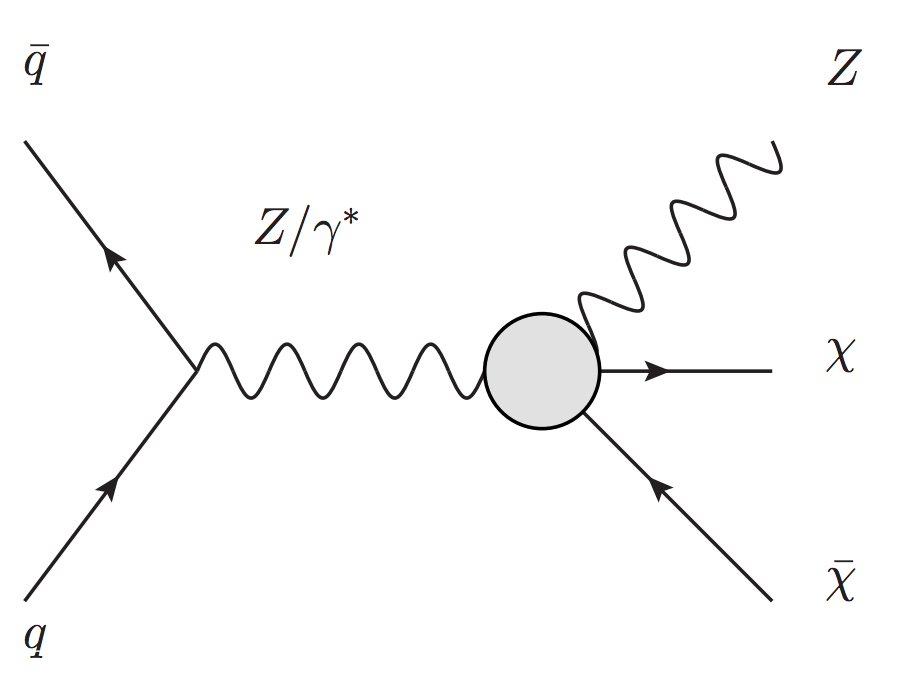
\includegraphics[width=\textwidth]{Figures/eft2.png}
        \label{fig:eft2}
    \end{subfigure}
    \caption{Representative EFT diagrams for the \monoZ signature \cite{Carpenter:2012rg}.}
\label{fig:efts}
\end{figure}

Leading order simplified models are the first set of benchmark models used for \etmissX searches in Run 2, as recommended by the LHC DM Working Group \cite{Boveia:2016mrp}. An example $s$-channel diagram for the \Zetmiss signal is shown in Figure \ref{fig:simp}. These models are considered `simplified' because they introduce the minimum number of parameters needed to include a mediator between SM and dark matter particles (compared to more complicated models such as supersymmetry). 

\begin{figure}[htb]
\centering
\selectcolormodel{gray}
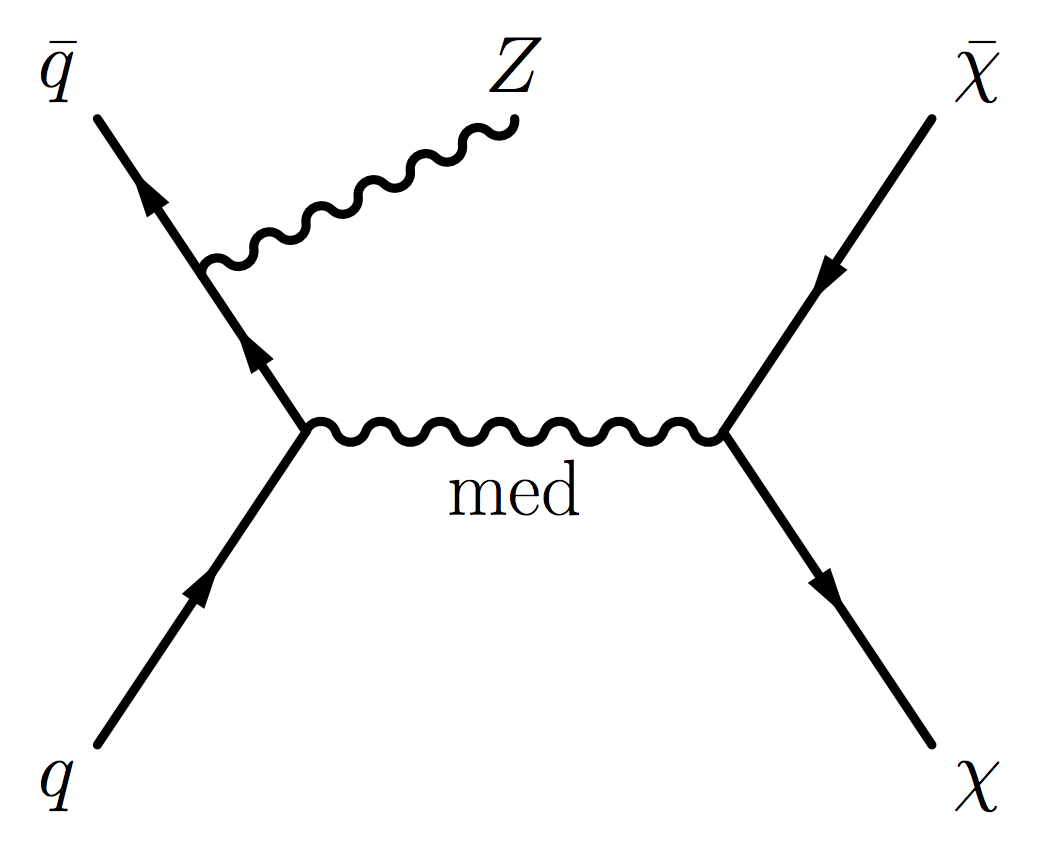
\includegraphics[width=0.3\textwidth]{Figures/simp.png}
\caption{Simplified model $s$-channel diagram for the \monoZ signature \cite{Aaboud:2017bja}.}
\label{fig:simp}
\end{figure}

Simplified models introduce five new parameters: the mass of the WIMP, \mchi, the mass of the mediating particle, \mmed, the couplings of the mediator to the SM (to dark matter), \gq (\gchi), and the width of the mediator \Wmed. The mediator particle can be spin-0 (scalar or pseudo-scalar) or spin-1 (vector or axial-vector). 

%The interaction Lagrangians for models with vector and axial-vector mediator couplings are given in Equations \ref{eqn:Lvector}, and \ref{eqn:Laxial}:

%\begin{equation}
%\mathcal{L}_\text{vector} = g_q \sum_q \eta_\mu \bar{q} \gamma^\mu q + g_\chi \eta_\mu \bar{\chi} \gamma^\mu \chi
%\label{eqn:Lvector}
%\end{equation}

%\begin{equation}
%\mathcal{L}_\text{axial-vector} = g_q \sum_q \eta_\mu \bar{q} \gamma^\mu \gamma^5 q + g_\chi \eta_\mu \bar{\chi} \gamma^\mu \gamma^5\chi
%\label{eqn:Laxial}
%\end{equation}

Following the recommendations in Ref.\ \cite{Boveia:2016mrp}, for spin-0 models the couplings are set to \gq~=~\gchi~=~1.0. The Yukawa couplings are also included between the quarks and the mediator. For spin-1 models the couplings are fixed to $g_q = 0.25$ and $g_\chi = 1.0$. In addition, assuming that the mediator has no additional decay modes, \Wmed is set to the minimal width \cite{Abercrombie:2015wmb}, which is fixed by \gq, \gchi, \mchi, and \mmed. The couplings were chosen so that \Wmed/\mmed < $\sim$0.05, and to correspond approximately to an estimate of the lower sensitivity of the Run 2 mono-jet analysis.

%Similarly, the interaction Lagrangians for models with scalar and pseudo-scalar mediator couplings are given by Equations \ref{eqn:Lscalar} and \ref{eqn:Lpseudo}:

%\begin{equation}
%\mathcal{L}_\text{scalar} = g_\chi \eta \bar{\chi} \chi + \frac{\eta}{\sqrt{2}} g_q \sum_i \left( y_i^u \bar{u}_i u_i + y_i^d \bar{d}_i d_i + y_i^\ell \bar{\ell}_i \ell_i \right)
%\label{eqn:Lscalar}
%\end{equation}

%\begin{equation}
%\mathcal{L}_\text{pseudo-scalar} = i g_\chi \eta \bar{\chi} \gamma_5 \chi + \frac{i \eta}{\sqrt{2}} g_q \sum_i \left( y_i^u \bar{u}_i \gamma_5 u_i + y_i^d \bar{d}_i \gamma_5 d_i + y_i^\ell \bar{\ell}_i \gamma_5 \ell_i \right)
%\label{eqn:Lpseudo}
%\end{equation}

% Assuming minimal flavour violation, spin-0 resonances will behave similarly to the Higgs boson (hence the Yukawa couplings)

Run 2 \monoX analyses have adopted the $s$-channel exchange of an axial-vector mediator as the primary benchmark scenario. This choice is motivated by the findings in Ref. \cite{Boveia:2016mrp} that show that collider searches can be more sensitive than direct detection experiments at low values of \mchi for this type of mediator. 

Although they have advantages compared to EFTs, simplified models are not a complete theory and violate unitarity for some regions of parameter space. At the beginning of Run 2 they were useful in providing a guideline for the ATLAS and CMS collaborations to follow in tandem, but there is now interest in studying richer, more theoretically complete models. 

\begin{figure}[htb]
\centering
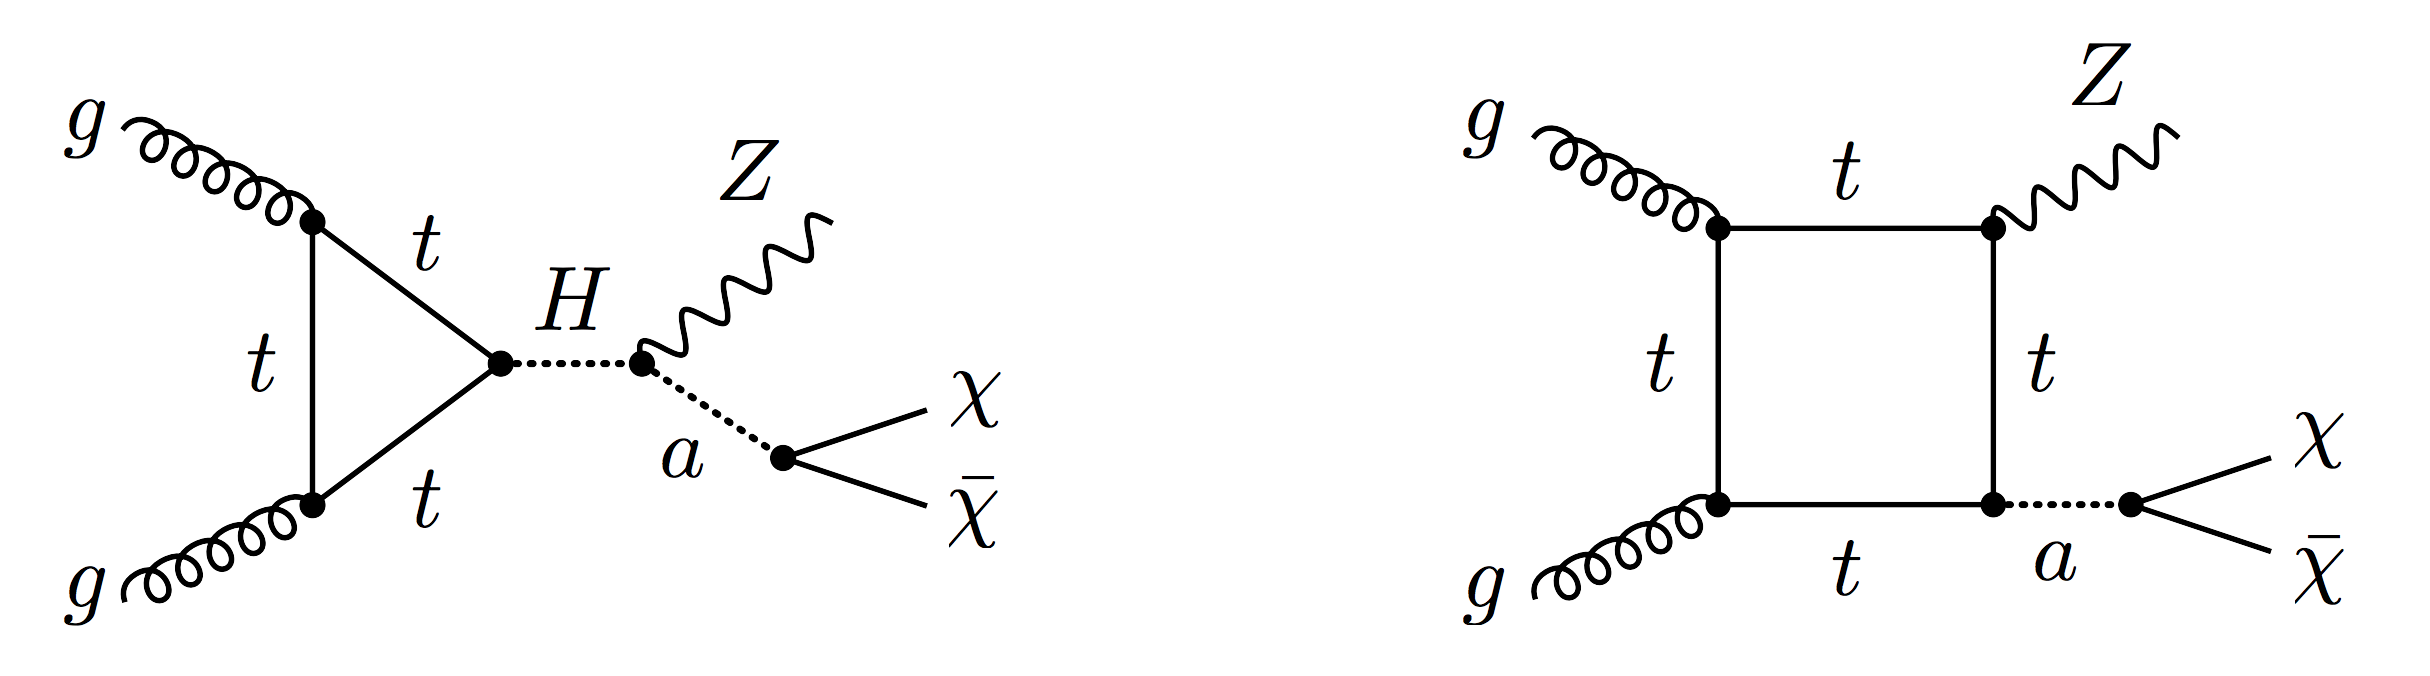
\includegraphics[width=0.75\textwidth]{Figures/2hdma.png}
\caption{2HDM+PS diagrams for the \monoZ signature produced by $gg$ fusion \cite{Bauer:2017ota}. The second diagram can have $A$ in place of $a$.}
\label{fig:2hdmaDiagrams}
\end{figure}

A popular model in Run 2 \monoX dark matter searches is known as the two Higgs doublet + pseudo-scalar (2HDM+PS) model \cite{Bauer:2017ota}. The addition of another SU(2) doublet to the SM is essential for many well-motivated BSM theories \cite{Branco:2011iw}. 2HDM models are also perturbative, and avoid violating unitarity by allowing mixing between the dark matter mediator and other bosons. 

Figure \ref{fig:2hdmaDiagrams} shows the two main diagrams of the 2HDM+PS model with the \monoZ signature. This model has two CP-even scalars $h$ and $H$ (where $h$ is the SM Higgs with $m_h$ = 125 GeV and $m_H > m_h$), one CP-odd pseudo-scalar $A$, two charged scalars $H^+$ and $H^-$, and the pseudo-scalar $a$ that couples the SM to dark matter. There are also the parameters $\sin(\beta-\alpha)$ and $\tan \beta$, where $\alpha$ is the mixing angle between $h$ and $H$, and $\tan \beta$ is the ratio of their vacuum expectation values. The parameters are chosen to have $m_A = m_H = m_{H^\pm}$.

Such models are of great interest to the \monoZ search because the \monoZ signature has better sensitivity than mono-jet for some regions of phase space. This is not the case for simplified models, where the mono-jet analysis always has higher sensitivity. In addition, there are couplings between $H$ and the $Z$ that are unique to the \monoZ search.

So far the \monoZ analysis has excluded a range of signals from the simplified and 2HDM+PS models. Prospective models to be studied with the full Run 2 dataset will be discussed in Chapter \ref{chapter:fullRun2}, including coloured scalar mediator ($t$-channel) signatures and so-called Less Simplified models.

\clearpage

% --------------------------------------------------------------------------------------
\section{The LHC and the ATLAS Detector}

The Large Hadron Collider (LHC) is the world's largest particle accelerator with a circumference of 27 km. Superconducting magnets are used to steer two beams of protons around the LHC as they are accelerated to nearly the speed of light. The beams are then brought to collision at various points around the LHC. Located at one of these collision points is the ATLAS detector, one of the two multipurpose detectors at the LHC. The LHC has been colliding protons at a centre-of-mass (COM) energy of 13 TeV since 2015, and ATLAS has been recording data.

The amount of \pp collision data delivered by the LHC is quantified by the \textit{luminosity}. The total number of $pp$ collisions $N$ detected over all time $t$ is related to the cross section for $pp$ collisions $\sigma$, and can be expressed in terms of either the instantaneous luminosity $L$ or the integrated luminosity $\mathcal{L}$:

\begin{equation}
N = \sigma \int{L} \text{d}t = \sigma \mathcal{L}
\end{equation}

\noindent $\mathcal{L}$ is the measure of total data collected that is frequently quoted in ATLAS. It has units of cm$^{-2}$, but a more frequently used unit is the inverse barn. 1 b = 10$^{-28}$ m$^2$. The total amount of data delivered by the LHC in the 2015-2017 period is 93 \ifb. ATLAS has recorded a total of 86 \ifb, with 80 \ifb that is good for physics analyses.

\begin{figure}[htb]
\centering
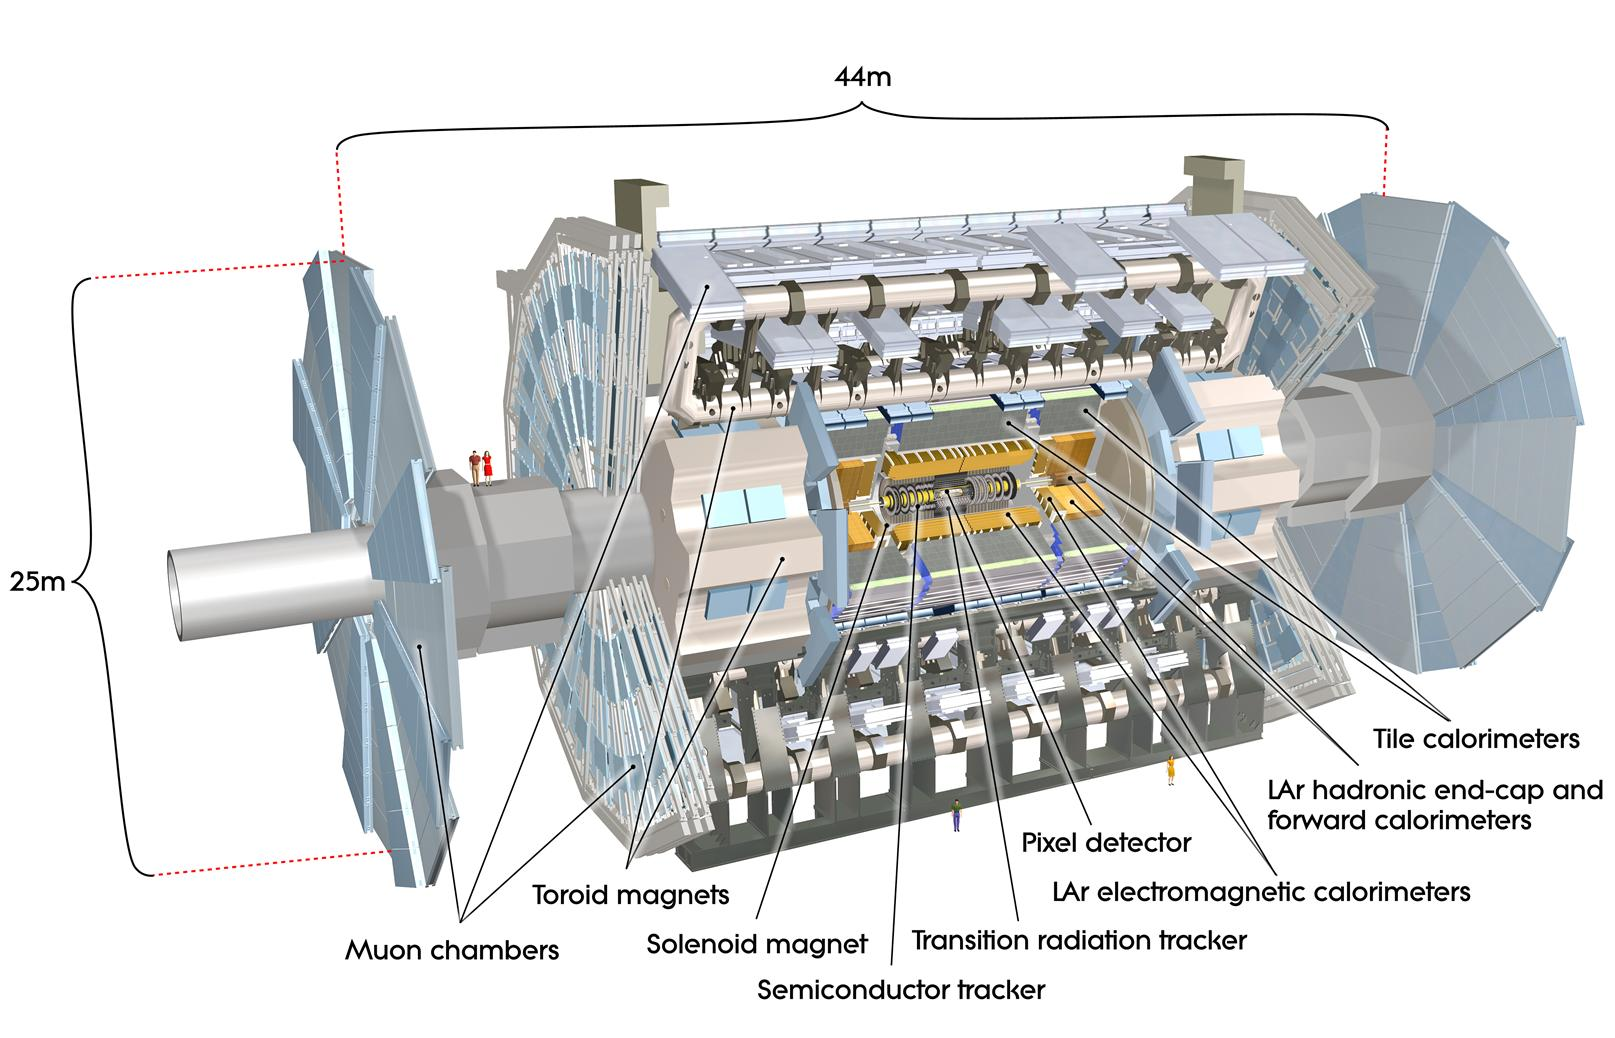
\includegraphics[width=1\textwidth]{Figures/atlas.jpg}
\caption{A cutaway view of the ATLAS detector with different subsystems labelled. The two humans on the left set the scale of the detector.}
\label{fig:atlas}
\end{figure}

An overview of the ATLAS detector is shown in Figure \ref{fig:atlas}. It is composed of four major subsystems. The innermost system is the inner detector which measures the tracks of charged particles very near to the collision point. It consists of three layers known as the pixel detector, semiconductor tracker, and transition radiation tracker. The innermost pixel detector has the highest resolution granularity in the detector and consists of 80 million pixels. The semiconductor tracker consists of 60 m$^2$ of silicon microstrips with densely packed readout channels, and the transition radiation tracker consists of 300,000 wires encased in straw tubes to measure tracks from ionization. The inner detector is encased in a solenoid that exerts a 2 Tesla magnetic field. The magnetic field causes the paths of charged particles to bend. The momentum of the particles can be determined from the curvature of the tracks.

Moving outward from the centre of the detector, the next subsystems are the electromagnetic and hadronic calorimeters. The electromagnetic system is entirely composed of liquid argon calorimetery, while the hadronic system includes the tile calorimeter in the barrel region and liquid argon calorimetry in the end-caps. The calorimeters are dense and designed to stop particles completely so that their energy is deposited entirely inside the detector. The electromagnetic calorimeter is designed to stop particles that interact electromagnetically (electrons and photons) while the hadronic calorimeter is designed to stop hadrons (e.g.\ protons and neutrons). The liquid argon calorimeter consists of alternating layers of copper absorber material and liquid argon ionization chambers, while the tile calorimeter alternates between layers of steel and plastic scintillators. 

The outermost and largest system of the detector is the muon spectrometer. Muons will interact minimally with the detector and so the spectrometer is designed to measure their momenta from tracks. The spectrometer consists of several systems. Monitored drift tubes are used in the barrel and end-caps for measuring track curvature. Resistive plate chambers, cathode strip chambers, and thin gap chambers are used for precision coordinate measurements throughout the spectrometer. The muon spectrometer also contains the ATLAS toroid magnet system.

Events that occur in the detector are recorded by the ATLAS trigger system. Due to the incredibly high rates of collisions inside the detector, it's not feasible to record every event that occurs (and most events are not interesting). The Level 1 trigger is hardware-based and makes decisions based on energy clusters in the calorimeter or coincidences in the muon spectrometer. If the event passes the Level 1 trigger, then it moves to the High Level Trigger, a more sophisticated software-based algorithm. A single electron trigger in the High Level Trigger may require, for example, that an object meets some electron identification criteria, has some minimum \pt, and is relatively isolated. The event is recorded to disk if the Level 1 and High Level Trigger selection criteria are satisfied.

\begin{figure}[!htb]
\centering
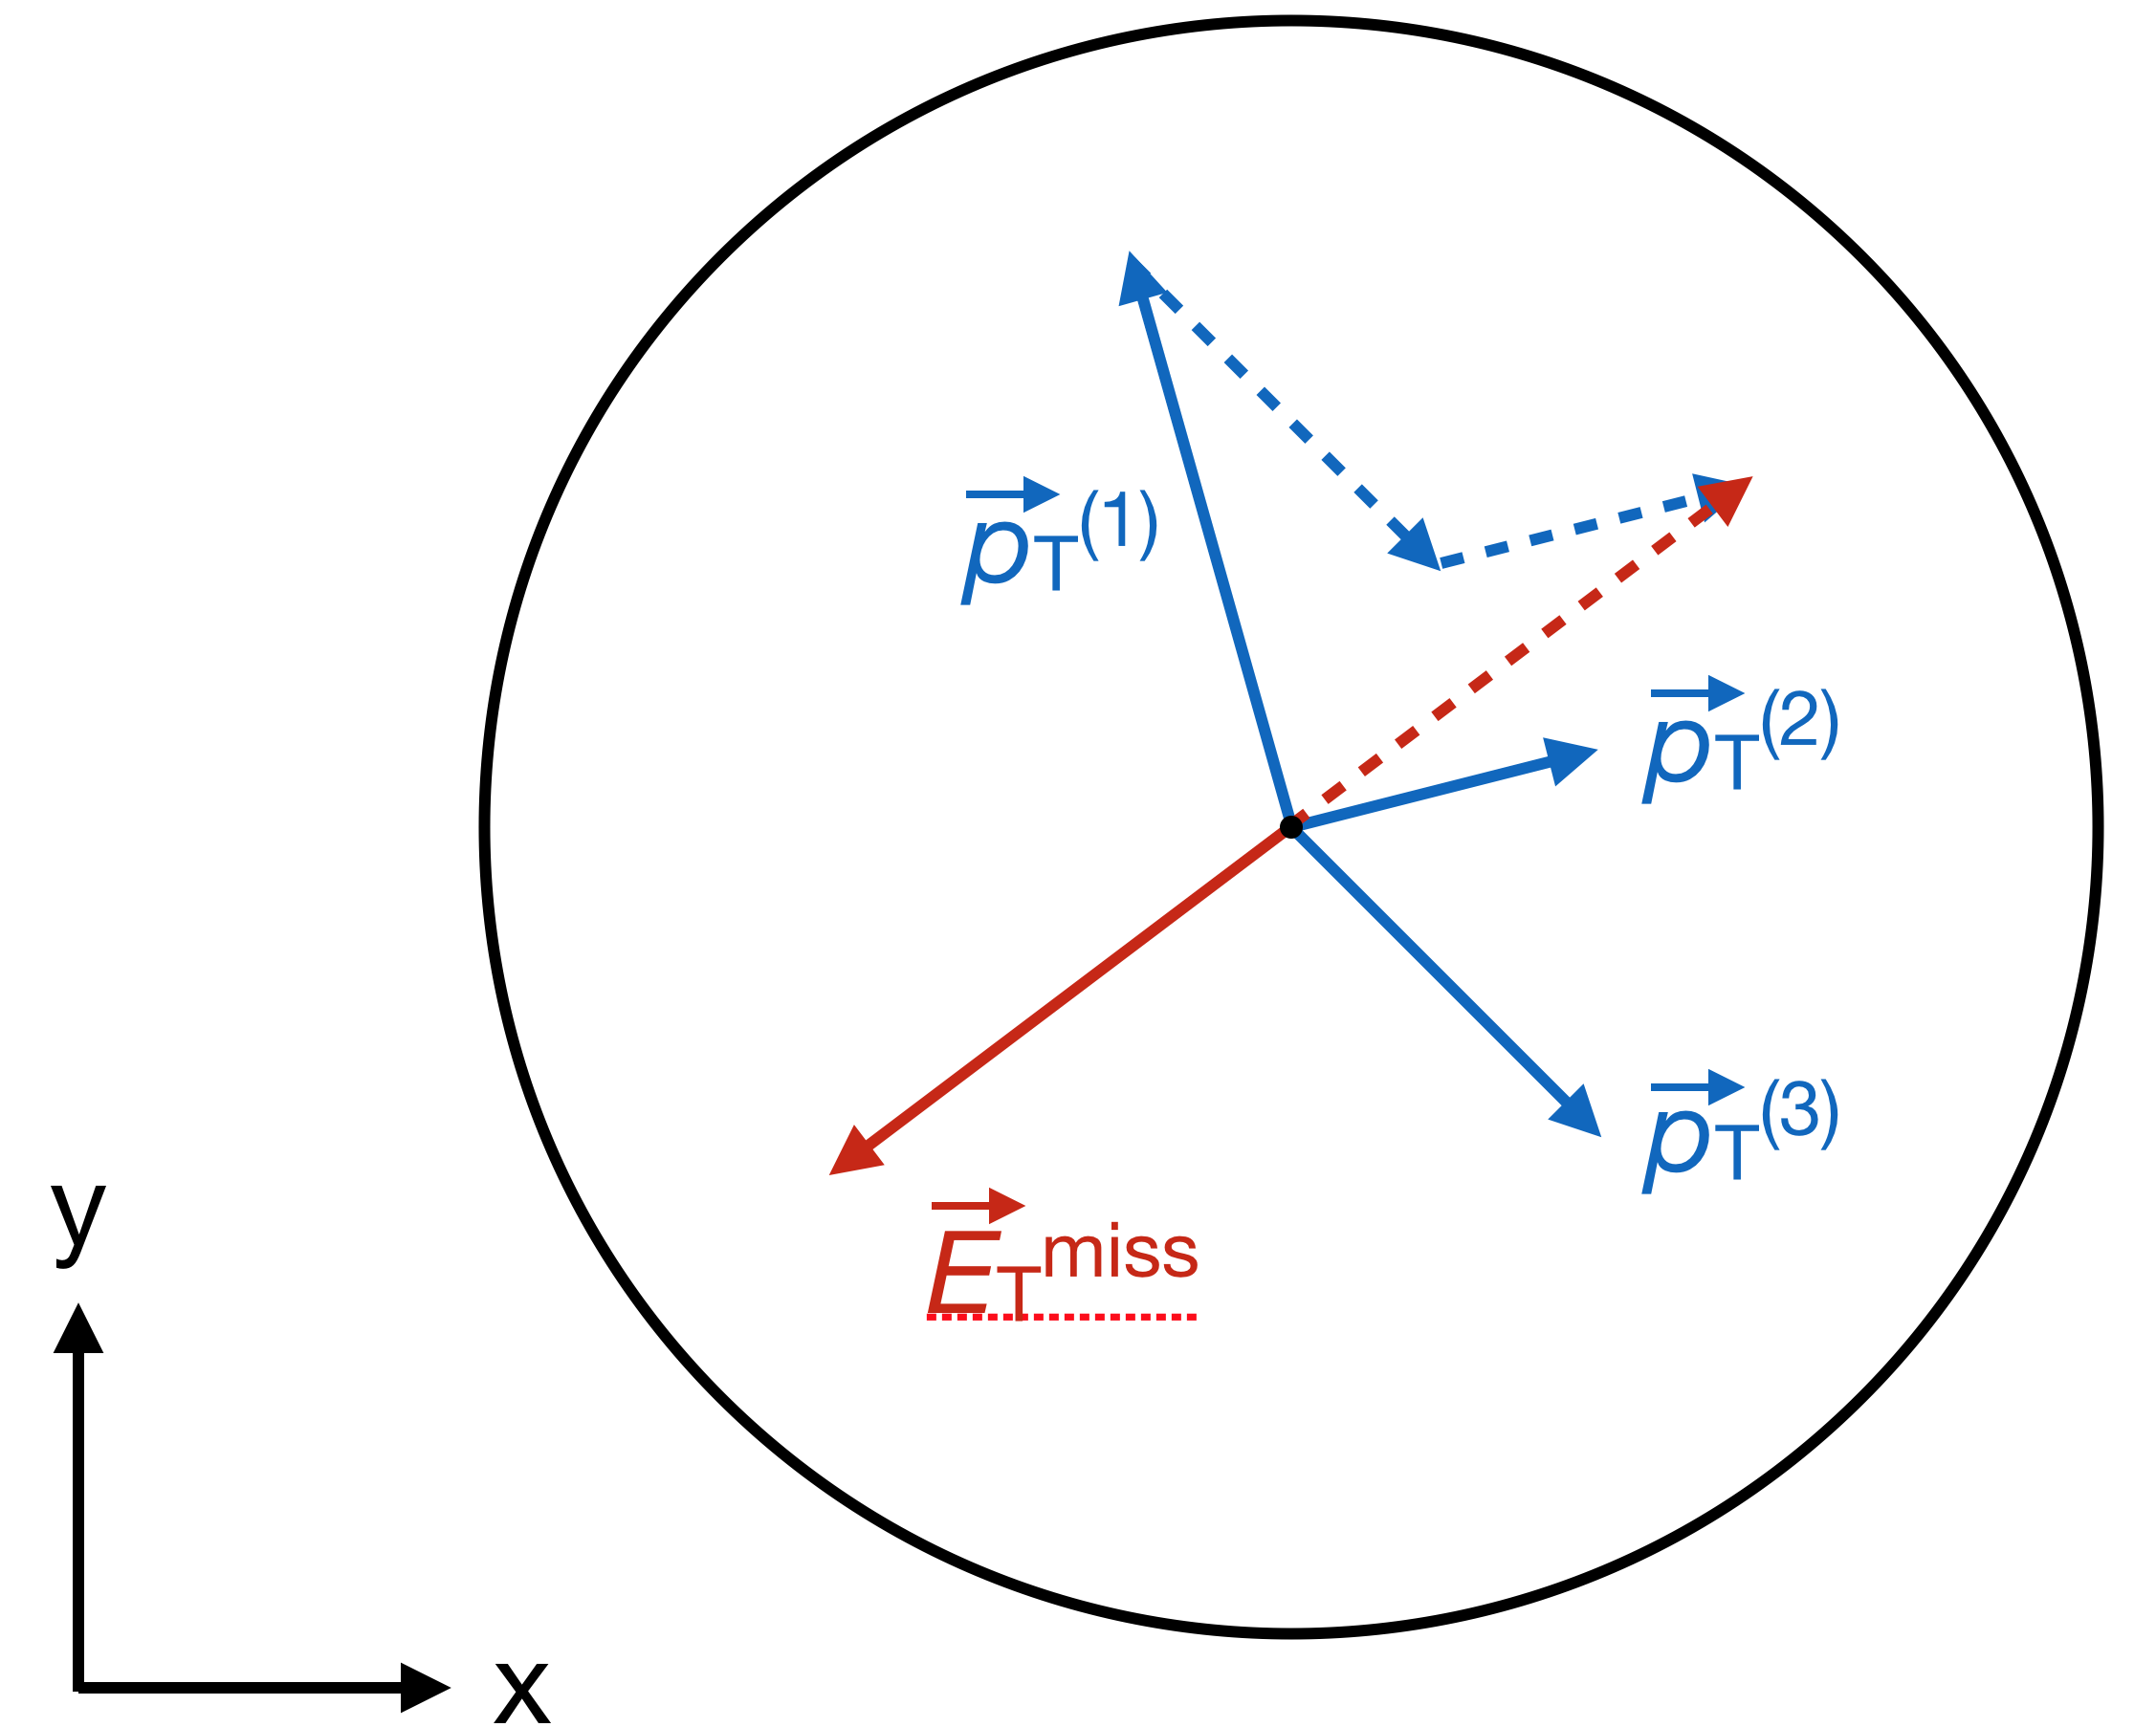
\includegraphics[width=0.4\textwidth]{Figures/etmiss.png}
\caption{Schematic of the missing transverse momentum \etmissvec.}
\label{fig:etmiss}
\end{figure}

Events that are recorded and deemed to be ``good for physics'' can be analyzed. The reconstructed objects in the events include electrons, photons, muons, and jets. The \etmiss is calculated using the reconstructed objects in the event. Figure \ref{fig:etmiss} shows an example of the transverse plane for an event with three measured particles. The \pt of the reconstructed objects in the event are added together (shown by the red dashed vector). Then the negative is taken to balance the measured \pt in the event (the solid red vector). This is the \etmissvec. The vector quantity \etmissvec is known as the missing transverse momentum, while its magnitude \etmiss is referred to as the missing transverse energy. The formal definition is given by:

\begin{equation}
\vec{E}_\text{T}^\text{miss} = - \left( \sum \vec{p}_\text{T}^\text{ jets} + \sum \vec{p}_\text{T}^\text{ electrons} + \sum \vec{p}_\text{T}^\text{ muons} + \sum \vec{p}_\text{T}^\text{ soft track} \right)
\end{equation}

\noindent The soft track term is formed from leftover tracks that are not used in reconstructed objects. Calorimeter energy clusters can also be used for this term, but tracks are more robust in high pileup environments. 

The physics objects used for a given analysis may have to satisfy further, stricter requirements, such as residing in a specific region of the detector. Then those selected objects are used to calculate the kinematic quantities used in the event selection.

\clearpage

